%*****************************************
\chapter{Future}\label{ch:future}
%*****************************************

\subsection{Recursive Loops and Infinite Recursive Tracing Descent}

If the focus on the tracing is controlled carefully, these potential
loops can be avoided.  How to detect and control these potential loops
is an interesting area of future automatic debugging research in
reflective control.

\subsection{Potential Future Uses for Low-Level Tracing}

Lower level objects maybe be interesting to focus on for research in
automatic abstraction and simulation of system components.  Optimizing
compilers could benefit from this area of future research.  E.g.
focusing on the CPU object could help to develop better run-time
register allocation models.

\subsection{Why Should You Use This Radically New Language?}

Because the language is very similar to Lisp, it has proven to be easy
for both expert and novice programmers to learn.  This has been my
experience with the four undergraduates that have worked within the
language, who learned it quickly, started writing their own macros to
facilitate their style, and one even made additions to the core
algorithms.

\section{Dealing with Noise in Agent Communication}

\begin{figure}[bth]
  \center
  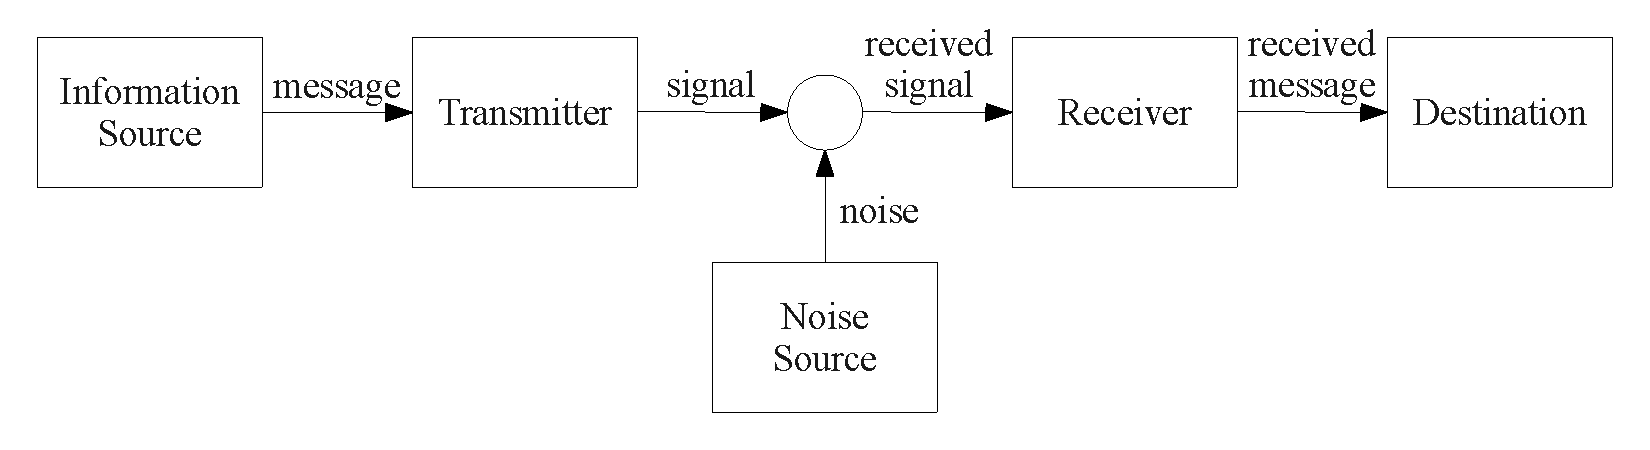
\includegraphics[width=10cm]{gfx/communication_theory}
  \caption[A theory of communication]{A theory of communication developed by Shannon~\citep{shannon:1959}.}
  \label{fig:communication_theory}
\end{figure}

Because agent processes can only directly act on and perceive the
environment, all communication between agent processes must occur
through the environment process.  Communication between agents in our
model occurs across a noiseless communication channel.  For extensions
of our model toward more realistic domains involving noisy
communication channels, Shannon's mathmematical theory of
communication~\citep{shannon:1959} can be applied.



